\documentclass[11pt, oneside]{article}   	% use "amsart" instead of "article" for AMSLaTeX format
\usepackage{geometry}                		% See geometry.pdf to learn the layout options. There are lots.
\geometry{letterpaper}                   		% ... or a4paper or a5paper or ... 
%\geometry{landscape}                		% Activate for for rotated page geometry
%\usepackage[parfill]{parskip}    		% Activate to begin paragraphs with an empty line rather than an indent
\usepackage{graphicx}				% Use pdf, png, jpg, or eps§ with pdflatex; use eps in DVI mode
								% TeX will automatically convert eps --> pdf in pdflatex		
\usepackage{amssymb}
\usepackage{amsmath}
\usepackage{parskip}
\usepackage{color}

\title{Kepler (part 1):  Newton}
%\author{The Author}
%\section{}
% \subsection*{R code}
\date{}							% Activate to display a given date or no date

\graphicspath{{/Users/telliott_admin/Dropbox/Tex/png/}}

% \begin{center} 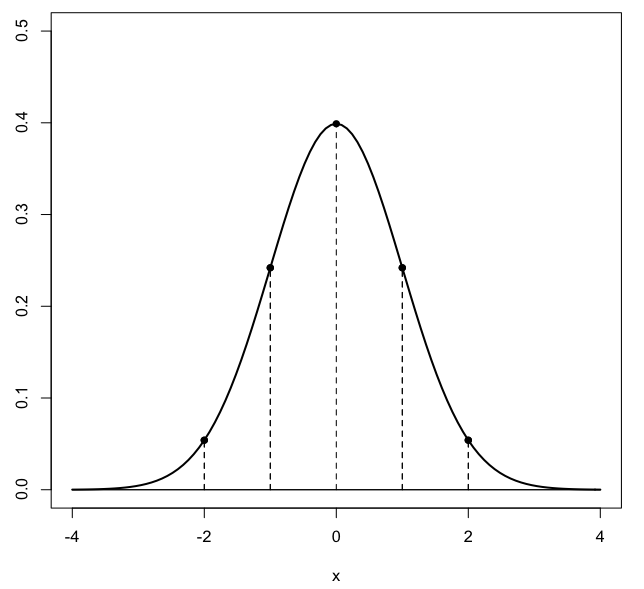
\includegraphics [scale=0.4] {gauss3.png} \end{center}

\begin{document}
\maketitle
\Large
\noindent

This is part two of ten, about deriving Kepler's Laws for planetary motion from Newton's Laws.  In this part, we look at the geometric proof of K2 used by Newton.
\begin{center} 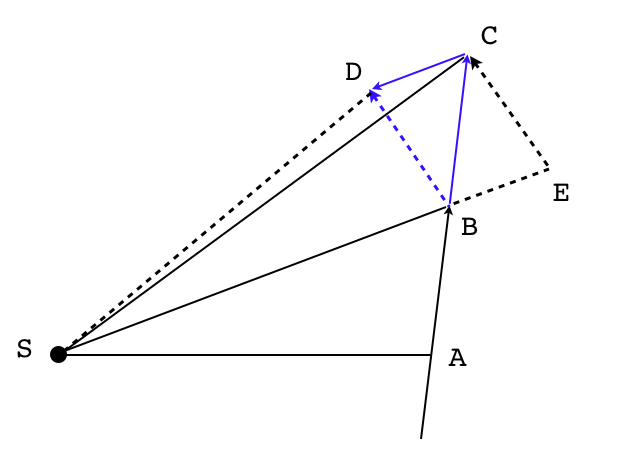
\includegraphics [scale=0.5] {newton_area.png} \end{center}
We diagram the sun $S$ and a planet at $A$.  Imagine that the force toward the sun is applied discretely.  That is, for a small interval $\Delta t$, the planet travels from $A$ to $B$ at constant velocity and if undisturbed, would travel to $C$ in the next unit of time.  

In the absence of a force, the velocity would be constant and so the length of $AB$ is the same as that of $BC$, and since $AB$ is on the same line as $BC$, the area of $\triangle ABS$ is equal to the area of $\triangle BCS$.  

Proof:  draw the vertical line from $S$ to the line containing $ABC$.  The area of either triangle is one-half the length of that altitude times the distance, either $AB$ or $BC$.  The principle is illustrated in the next figure.
\begin{center} 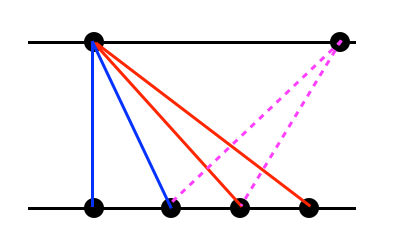
\includegraphics [scale=0.5] {triangles_parallel.png} \end{center}
Given two parallel lines separated by a distance $h$, pick two points on one line separated by a distance $d$ and \emph{any} point on the other line.  The triangles drawn using those points will all have equal area, namely $(1/2)dh$.

Now, suppose the force is applied at $B$ \emph{toward the sun} along $EBS$.  As a result, the trajectory $BC$ is modified by the change in velocity resulting from application of the force toward the sun. The new path is the additional velocity times $\Delta t$.  Call the length $CD$ and add it to $BC$ to give the actual trajectory, $BD$.  

$CD$ is parallel to $SBE$.  Therefore, every point on $CD$ has an altitude with respect to $SBE$ of the same length.  So any point on $CD$ can be used to draw a triangle with the same base $SB$ and the result will have the equal area no matter which point is chosen.

In particular, the area of $\triangle BDS$ is equal to the area of $\triangle BCS$, which was found earlier to be equal to the area of $\triangle ABS$.  Since the two triangles from the actual motion have the same area, the area is constant.
\end{document}  